\documentclass[1p]{elsarticle_modified}
%\bibliographystyle{elsarticle-num}

%\usepackage[colorlinks]{hyperref}
%\usepackage{abbrmath_seonhwa} %\Abb, \Ascr, \Acal ,\Abf, \Afrak
\usepackage{amsfonts}
\usepackage{amssymb}
\usepackage{amsmath}
\usepackage{amsthm}
\usepackage{scalefnt}
\usepackage{amsbsy}
\usepackage{kotex}
\usepackage{caption}
\usepackage{subfig}
\usepackage{color}
\usepackage{graphicx}
\usepackage{xcolor} %% white, black, red, green, blue, cyan, magenta, yellow
\usepackage{float}
\usepackage{setspace}
\usepackage{hyperref}

\usepackage{tikz}
\usetikzlibrary{arrows}

\usepackage{multirow}
\usepackage{array} % fixed length table
\usepackage{hhline}

%%%%%%%%%%%%%%%%%%%%%
\makeatletter
\renewcommand*\env@matrix[1][\arraystretch]{%
	\edef\arraystretch{#1}%
	\hskip -\arraycolsep
	\let\@ifnextchar\new@ifnextchar
	\array{*\c@MaxMatrixCols c}}
\makeatother %https://tex.stackexchange.com/questions/14071/how-can-i-increase-the-line-spacing-in-a-matrix
%%%%%%%%%%%%%%%

\usepackage[normalem]{ulem}

\newcommand{\msout}[1]{\ifmmode\text{\sout{\ensuremath{#1}}}\else\sout{#1}\fi}
%SOURCE: \msout is \stkout macro in https://tex.stackexchange.com/questions/20609/strikeout-in-math-mode

\newcommand{\cancel}[1]{
	\ifmmode
	{\color{red}\msout{#1}}
	\else
	{\color{red}\sout{#1}}
	\fi
}

\newcommand{\add}[1]{
	{\color{blue}\uwave{#1}}
}

\newcommand{\replace}[2]{
	\ifmmode
	{\color{red}\msout{#1}}{\color{blue}\uwave{#2}}
	\else
	{\color{red}\sout{#1}}{\color{blue}\uwave{#2}}
	\fi
}

\newcommand{\Sol}{\mathcal{S}} %segment
\newcommand{\D}{D} %diagram
\newcommand{\A}{\mathcal{A}} %arc


%%%%%%%%%%%%%%%%%%%%%%%%%%%%%5 test

\def\sl{\operatorname{\textup{SL}}(2,\Cbb)}
\def\psl{\operatorname{\textup{PSL}}(2,\Cbb)}
\def\quan{\mkern 1mu \triangleright \mkern 1mu}

\theoremstyle{definition}
\newtheorem{thm}{Theorem}[section]
\newtheorem{prop}[thm]{Proposition}
\newtheorem{lem}[thm]{Lemma}
\newtheorem{ques}[thm]{Question}
\newtheorem{cor}[thm]{Corollary}
\newtheorem{defn}[thm]{Definition}
\newtheorem{exam}[thm]{Example}
\newtheorem{rmk}[thm]{Remark}
\newtheorem{alg}[thm]{Algorithm}

\newcommand{\I}{\sqrt{-1}}
\begin{document}

%\begin{frontmatter}
%
%\title{Boundary parabolic representations of knots up to 8 crossings}
%
%%% Group authors per affiliation:
%\author{Yunhi Cho} 
%\address{Department of Mathematics, University of Seoul, Seoul, Korea}
%\ead{yhcho@uos.ac.kr}
%
%
%\author{Seonhwa Kim} %\fnref{s_kim}}
%\address{Center for Geometry and Physics, Institute for Basic Science, Pohang, 37673, Korea}
%\ead{ryeona17@ibs.re.kr}
%
%\author{Hyuk Kim}
%\address{Department of Mathematical Sciences, Seoul National University, Seoul 08826, Korea}
%\ead{hyukkim@snu.ac.kr}
%
%\author{Seokbeom Yoon}
%\address{Department of Mathematical Sciences, Seoul National University, Seoul, 08826,  Korea}
%\ead{sbyoon15@snu.ac.kr}
%
%\begin{abstract}
%We find all boundary parabolic representation of knots up to 8 crossings.
%
%\end{abstract}
%\begin{keyword}
%    \MSC[2010] 57M25 
%\end{keyword}
%
%\end{frontmatter}

%\linenumbers
%\tableofcontents
%
\newcommand\colored[1]{\textcolor{white}{\rule[-0.35ex]{0.8em}{1.4ex}}\kern-0.8em\color{red} #1}%
%\newcommand\colored[1]{\textcolor{white}{ #1}\kern-2.17ex	\textcolor{white}{ #1}\kern-1.81ex	\textcolor{white}{ #1}\kern-2.15ex\color{red}#1	}

{\Large $\underline{12a_{1069}~(K12a_{1069})}$}

\setlength{\tabcolsep}{10pt}
\renewcommand{\arraystretch}{1.6}
\vspace{1cm}\begin{tabular}{m{100pt}>{\centering\arraybackslash}m{274pt}}
\multirow{5}{120pt}{
	\centering
	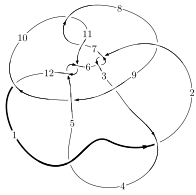
\includegraphics[width=112pt]{../../../GIT/diagram.site/Diagrams/png/1870_12a_1069.png}\\
\ \ \ A knot diagram\footnotemark}&
\allowdisplaybreaks
\textbf{Linearized knot diagam} \\
\cline{2-2}
 &
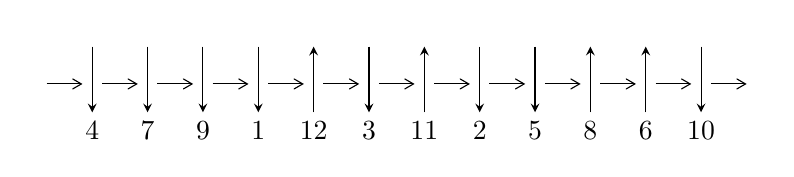
\begin{tikzpicture}[x=20pt, y=17pt]
	% nodes
	\node (C0) at (0, 0) {};
	\node (C1) at (1, 0) {};
	\node (C1U) at (1, +1) {};
	\node (C1D) at (1, -1) {4};

	\node (C2) at (2, 0) {};
	\node (C2U) at (2, +1) {};
	\node (C2D) at (2, -1) {7};

	\node (C3) at (3, 0) {};
	\node (C3U) at (3, +1) {};
	\node (C3D) at (3, -1) {9};

	\node (C4) at (4, 0) {};
	\node (C4U) at (4, +1) {};
	\node (C4D) at (4, -1) {1};

	\node (C5) at (5, 0) {};
	\node (C5U) at (5, +1) {};
	\node (C5D) at (5, -1) {12};

	\node (C6) at (6, 0) {};
	\node (C6U) at (6, +1) {};
	\node (C6D) at (6, -1) {3};

	\node (C7) at (7, 0) {};
	\node (C7U) at (7, +1) {};
	\node (C7D) at (7, -1) {11};

	\node (C8) at (8, 0) {};
	\node (C8U) at (8, +1) {};
	\node (C8D) at (8, -1) {2};

	\node (C9) at (9, 0) {};
	\node (C9U) at (9, +1) {};
	\node (C9D) at (9, -1) {5};

	\node (C10) at (10, 0) {};
	\node (C10U) at (10, +1) {};
	\node (C10D) at (10, -1) {8};

	\node (C11) at (11, 0) {};
	\node (C11U) at (11, +1) {};
	\node (C11D) at (11, -1) {6};

	\node (C12) at (12, 0) {};
	\node (C12U) at (12, +1) {};
	\node (C12D) at (12, -1) {10};
	\node (C13) at (13, 0) {};

	% arrows
	\draw[->,>={angle 60}]
	(C0) edge (C1) (C1) edge (C2) (C2) edge (C3) (C3) edge (C4) (C4) edge (C5) (C5) edge (C6) (C6) edge (C7) (C7) edge (C8) (C8) edge (C9) (C9) edge (C10) (C10) edge (C11) (C11) edge (C12) (C12) edge (C13) ;	\draw[->,>=stealth]
	(C1U) edge (C1D) (C2U) edge (C2D) (C3U) edge (C3D) (C4U) edge (C4D) (C5D) edge (C5U) (C6U) edge (C6D) (C7D) edge (C7U) (C8U) edge (C8D) (C9U) edge (C9D) (C10D) edge (C10U) (C11D) edge (C11U) (C12U) edge (C12D) ;
	\end{tikzpicture} \\
\hhline{~~} \\& 
\textbf{Solving Sequence} \\ \cline{2-2} 
 &
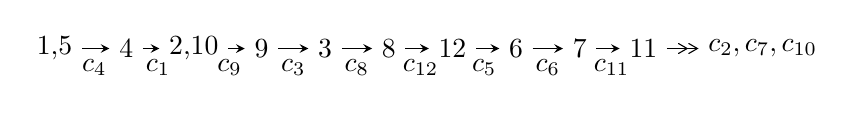
\begin{tikzpicture}[x=23pt, y=7pt]
	% node
	\node (A0) at (-1/8, 0) {1,5};
	\node (A1) at (1, 0) {4};
	\node (A2) at (33/16, 0) {2,10};
	\node (A3) at (25/8, 0) {9};
	\node (A4) at (33/8, 0) {3};
	\node (A5) at (41/8, 0) {8};
	\node (A6) at (49/8, 0) {12};
	\node (A7) at (57/8, 0) {6};
	\node (A8) at (65/8, 0) {7};
	\node (A9) at (73/8, 0) {11};
	\node (C1) at (1/2, -1) {$c_{4}$};
	\node (C2) at (3/2, -1) {$c_{1}$};
	\node (C3) at (21/8, -1) {$c_{9}$};
	\node (C4) at (29/8, -1) {$c_{3}$};
	\node (C5) at (37/8, -1) {$c_{8}$};
	\node (C6) at (45/8, -1) {$c_{12}$};
	\node (C7) at (53/8, -1) {$c_{5}$};
	\node (C8) at (61/8, -1) {$c_{6}$};
	\node (C9) at (69/8, -1) {$c_{11}$};
	\node (A10) at (11, 0) {$c_{2},c_{7},c_{10}$};

	% edge
	\draw[->,>=stealth]	
	(A0) edge (A1) (A1) edge (A2) (A2) edge (A3) (A3) edge (A4) (A4) edge (A5) (A5) edge (A6) (A6) edge (A7) (A7) edge (A8) (A8) edge (A9) ;
	\draw[->>,>={angle 60}]	
	(A9) edge (A10);
\end{tikzpicture} \\ 

\end{tabular} \\

\footnotetext{
The image of knot diagram is generated by the software ``\textbf{Draw programme}" developed by Andrew Bartholomew(\url{http://www.layer8.co.uk/maths/draw/index.htm\#Running-draw}), where we modified some parts for our purpose(\url{https://github.com/CATsTAILs/LinksPainter}).
}\phantom \\ \newline 
\centering \textbf{Ideals for irreducible components\footnotemark of $X_{\text{par}}$} 
 
\begin{align*}
I^u_{1}&=\langle 
-3.51005\times10^{774} u^{158}+1.44047\times10^{775} u^{157}+\cdots+1.24689\times10^{774} b+4.06181\times10^{776},\\
\phantom{I^u_{1}}&\phantom{= \langle  }-3.52571\times10^{776} u^{158}+1.70406\times10^{777} u^{157}+\cdots+5.11223\times10^{775} a+8.33651\times10^{778},\\
\phantom{I^u_{1}}&\phantom{= \langle  }u^{159}-5 u^{158}+\cdots-1836 u+41\rangle \\
I^u_{2}&=\langle 
-1.15427\times10^{39} u^{41}-3.52555\times10^{39} u^{40}+\cdots+2.16791\times10^{39} b+3.15442\times10^{39},\\
\phantom{I^u_{2}}&\phantom{= \langle  }-1.18323\times10^{38} u^{41}+1.54707\times10^{39} u^{40}+\cdots+3.68545\times10^{40} a+4.04012\times10^{41},\\
\phantom{I^u_{2}}&\phantom{= \langle  }u^{42}+4 u^{41}+\cdots+81 u+17\rangle \\
\\
\end{align*}
\raggedright * 2 irreducible components of $\dim_{\mathbb{C}}=0$, with total 201 representations.\\
\footnotetext{All coefficients of polynomials are rational numbers. But the coefficients are sometimes approximated in decimal forms when there is not enough margin.}
\newpage
\renewcommand{\arraystretch}{1}
\centering \section*{I. $I^u_{1}= \langle -3.51\times10^{774} u^{158}+1.44\times10^{775} u^{157}+\cdots+1.25\times10^{774} b+4.06\times10^{776},\;-3.53\times10^{776} u^{158}+1.70\times10^{777} u^{157}+\cdots+5.11\times10^{775} a+8.34\times10^{778},\;u^{159}-5 u^{158}+\cdots-1836 u+41 \rangle$}
\flushleft \textbf{(i) Arc colorings}\\
\begin{tabular}{m{7pt} m{180pt} m{7pt} m{180pt} }
\flushright $a_{1}=$&$\begin{pmatrix}0\\u\end{pmatrix}$ \\
\flushright $a_{5}=$&$\begin{pmatrix}1\\0\end{pmatrix}$ \\
\flushright $a_{4}=$&$\begin{pmatrix}1\\- u^2\end{pmatrix}$ \\
\flushright $a_{2}=$&$\begin{pmatrix}- u\\u^3+u\end{pmatrix}$ \\
\flushright $a_{10}=$&$\begin{pmatrix}6.89661 u^{158}-33.3329 u^{157}+\cdots+62395.2 u-1630.70\\2.81505 u^{158}-11.5525 u^{157}+\cdots+12205.5 u-325.757\end{pmatrix}$ \\
\flushright $a_{9}=$&$\begin{pmatrix}9.71167 u^{158}-44.8855 u^{157}+\cdots+74600.7 u-1956.46\\2.81505 u^{158}-11.5525 u^{157}+\cdots+12205.5 u-325.757\end{pmatrix}$ \\
\flushright $a_{3}=$&$\begin{pmatrix}12.2156 u^{158}-58.2653 u^{157}+\cdots+118758. u-2988.83\\-0.707859 u^{158}+4.12082 u^{157}+\cdots-1849.09 u+41.7737\end{pmatrix}$ \\
\flushright $a_{8}=$&$\begin{pmatrix}9.18241 u^{158}-43.6668 u^{157}+\cdots+78859.8 u-2060.49\\2.35801 u^{158}-9.73562 u^{157}+\cdots+10545.6 u-280.259\end{pmatrix}$ \\
\flushright $a_{12}=$&$\begin{pmatrix}-8.75638 u^{158}+42.9843 u^{157}+\cdots-81724.3 u+2101.75\\-2.38010 u^{158}+12.1412 u^{157}+\cdots-20129.1 u+507.031\end{pmatrix}$ \\
\flushright $a_{6}=$&$\begin{pmatrix}8.53022 u^{158}-41.2871 u^{157}+\cdots+59998.2 u-1469.69\\-1.94140 u^{158}+9.07101 u^{157}+\cdots-15520.2 u+397.134\end{pmatrix}$ \\
\flushright $a_{7}=$&$\begin{pmatrix}10.0548 u^{158}-50.2105 u^{157}+\cdots+95588.8 u-2414.43\\0.727499 u^{158}-4.63539 u^{157}+\cdots+16528.9 u-415.930\end{pmatrix}$ \\
\flushright $a_{11}=$&$\begin{pmatrix}14.1659 u^{158}-70.1808 u^{157}+\cdots+124297. u-3139.38\\0.119106 u^{158}+0.550360 u^{157}+\cdots-1796.57 u+44.4550\end{pmatrix}$\\&\end{tabular}
\flushleft \textbf{(ii) Obstruction class $= -1$}\\~\\
\flushleft \textbf{(iii) Cusp Shapes $= -6.97728 u^{158}+30.2719 u^{157}+\cdots-100238. u+2580.10$}\\~\\
\newpage\renewcommand{\arraystretch}{1}
\flushleft \textbf{(iv) u-Polynomials at the component}\newline \\
\begin{tabular}{m{50pt}|m{274pt}}
Crossings & \hspace{64pt}u-Polynomials at each crossing \\
\hline $$\begin{aligned}c_{1},c_{4}\end{aligned}$$&$\begin{aligned}
&u^{159}-5 u^{158}+\cdots-1836 u+41
\end{aligned}$\\
\hline $$\begin{aligned}c_{2},c_{6}\end{aligned}$$&$\begin{aligned}
&u^{159}+5 u^{158}+\cdots+1580 u+304
\end{aligned}$\\
\hline $$\begin{aligned}c_{3}\end{aligned}$$&$\begin{aligned}
&u^{159}+u^{158}+\cdots+107562 u+9857
\end{aligned}$\\
\hline $$\begin{aligned}c_{5},c_{11}\end{aligned}$$&$\begin{aligned}
&u^{159}- u^{158}+\cdots+76831096 u+4906757
\end{aligned}$\\
\hline $$\begin{aligned}c_{7},c_{10}\end{aligned}$$&$\begin{aligned}
&u^{159}-13 u^{158}+\cdots+677715 u+119125
\end{aligned}$\\
\hline $$\begin{aligned}c_{8}\end{aligned}$$&$\begin{aligned}
&u^{159}- u^{158}+\cdots+186934042 u+51574948
\end{aligned}$\\
\hline $$\begin{aligned}c_{9}\end{aligned}$$&$\begin{aligned}
&u^{159}-3 u^{158}+\cdots-52 u+4
\end{aligned}$\\
\hline $$\begin{aligned}c_{12}\end{aligned}$$&$\begin{aligned}
&u^{159}-11 u^{158}+\cdots+267 u-7
\end{aligned}$\\
\hline
\end{tabular}\\~\\
\newpage\renewcommand{\arraystretch}{1}
\flushleft \textbf{(v) Riley Polynomials at the component}\newline \\
\begin{tabular}{m{50pt}|m{274pt}}
Crossings & \hspace{64pt}Riley Polynomials at each crossing \\
\hline $$\begin{aligned}c_{1},c_{4}\end{aligned}$$&$\begin{aligned}
&y^{159}+115 y^{158}+\cdots+133618 y-1681
\end{aligned}$\\
\hline $$\begin{aligned}c_{2},c_{6}\end{aligned}$$&$\begin{aligned}
&y^{159}+77 y^{158}+\cdots-4109520 y-92416
\end{aligned}$\\
\hline $$\begin{aligned}c_{3}\end{aligned}$$&$\begin{aligned}
&y^{159}+29 y^{158}+\cdots-3124719192 y-97160449
\end{aligned}$\\
\hline $$\begin{aligned}c_{5},c_{11}\end{aligned}$$&$\begin{aligned}
&y^{159}+121 y^{158}+\cdots-799516959728630 y-24076264257049
\end{aligned}$\\
\hline $$\begin{aligned}c_{7},c_{10}\end{aligned}$$&$\begin{aligned}
&y^{159}+89 y^{158}+\cdots-542898621275 y-14190765625
\end{aligned}$\\
\hline $$\begin{aligned}c_{8}\end{aligned}$$&$\begin{aligned}
&y^{159}+37 y^{158}+\cdots-77763978165498852 y-2659975261202704
\end{aligned}$\\
\hline $$\begin{aligned}c_{9}\end{aligned}$$&$\begin{aligned}
&y^{159}- y^{158}+\cdots+232 y-16
\end{aligned}$\\
\hline $$\begin{aligned}c_{12}\end{aligned}$$&$\begin{aligned}
&y^{159}-3 y^{158}+\cdots-1021 y-49
\end{aligned}$\\
\hline
\end{tabular}\\~\\
\newpage\flushleft \textbf{(vi) Complex Volumes and Cusp Shapes}
$$\begin{array}{c|c|c}  
\text{Solutions to }I^u_{1}& \I (\text{vol} + \sqrt{-1}CS) & \text{Cusp shape}\\
 \hline 
\begin{aligned}
u &= -0.983003 + 0.097556 I \\
a &= -0.905981 + 0.783265 I \\
b &= \phantom{-}0.934039 - 0.432894 I\end{aligned}
 & -3.48952 + 3.13704 I & \phantom{-0.000000 } 0 \\ \hline\begin{aligned}
u &= -0.983003 - 0.097556 I \\
a &= -0.905981 - 0.783265 I \\
b &= \phantom{-}0.934039 + 0.432894 I\end{aligned}
 & -3.48952 - 3.13704 I & \phantom{-0.000000 } 0 \\ \hline\begin{aligned}
u &= \phantom{-}0.262735 + 0.984218 I \\
a &= \phantom{-}0.16813 + 2.67086 I \\
b &= \phantom{-}0.207483 - 0.022035 I\end{aligned}
 & -1.89883 - 9.65845 I & \phantom{-0.000000 } 0 \\ \hline\begin{aligned}
u &= \phantom{-}0.262735 - 0.984218 I \\
a &= \phantom{-}0.16813 - 2.67086 I \\
b &= \phantom{-}0.207483 + 0.022035 I\end{aligned}
 & -1.89883 + 9.65845 I & \phantom{-0.000000 } 0 \\ \hline\begin{aligned}
u &= -0.072291 + 1.016920 I \\
a &= \phantom{-}1.84966 - 0.36433 I \\
b &= -1.183920 - 0.349302 I\end{aligned}
 & -2.19049 - 2.79781 I & \phantom{-0.000000 } 0 \\ \hline\begin{aligned}
u &= -0.072291 - 1.016920 I \\
a &= \phantom{-}1.84966 + 0.36433 I \\
b &= -1.183920 + 0.349302 I\end{aligned}
 & -2.19049 + 2.79781 I & \phantom{-0.000000 } 0 \\ \hline\begin{aligned}
u &= -0.652432 + 0.783430 I \\
a &= -0.830407 + 0.000594 I \\
b &= \phantom{-}0.110772 - 0.942984 I\end{aligned}
 & -0.00445 + 3.94039 I & \phantom{-0.000000 } 0 \\ \hline\begin{aligned}
u &= -0.652432 - 0.783430 I \\
a &= -0.830407 - 0.000594 I \\
b &= \phantom{-}0.110772 + 0.942984 I\end{aligned}
 & -0.00445 - 3.94039 I & \phantom{-0.000000 } 0 \\ \hline\begin{aligned}
u &= -0.950490 + 0.166511 I \\
a &= -1.126060 + 0.618081 I \\
b &= \phantom{-}1.032190 - 0.478096 I\end{aligned}
 & -3.92600 + 3.26823 I & \phantom{-0.000000 } 0 \\ \hline\begin{aligned}
u &= -0.950490 - 0.166511 I \\
a &= -1.126060 - 0.618081 I \\
b &= \phantom{-}1.032190 + 0.478096 I\end{aligned}
 & -3.92600 - 3.26823 I & \phantom{-0.000000 } 0\\
 \hline 
 \end{array}$$\newpage$$\begin{array}{c|c|c}  
\text{Solutions to }I^u_{1}& \I (\text{vol} + \sqrt{-1}CS) & \text{Cusp shape}\\
 \hline 
\begin{aligned}
u &= -0.851291 + 0.434377 I \\
a &= \phantom{-}0.311298 + 0.923022 I \\
b &= -1.042790 - 0.658033 I\end{aligned}
 & -5.65361 - 5.39741 I & \phantom{-0.000000 } 0 \\ \hline\begin{aligned}
u &= -0.851291 - 0.434377 I \\
a &= \phantom{-}0.311298 - 0.923022 I \\
b &= -1.042790 + 0.658033 I\end{aligned}
 & -5.65361 + 5.39741 I & \phantom{-0.000000 } 0 \\ \hline\begin{aligned}
u &= \phantom{-}0.934381 + 0.185617 I \\
a &= \phantom{-}1.184470 + 0.642059 I \\
b &= -1.090390 - 0.698765 I\end{aligned}
 & -1.86192 - 7.90269 I & \phantom{-0.000000 } 0 \\ \hline\begin{aligned}
u &= \phantom{-}0.934381 - 0.185617 I \\
a &= \phantom{-}1.184470 - 0.642059 I \\
b &= -1.090390 + 0.698765 I\end{aligned}
 & -1.86192 + 7.90269 I & \phantom{-0.000000 } 0 \\ \hline\begin{aligned}
u &= -0.847254 + 0.622429 I \\
a &= -1.63548 + 0.29444 I \\
b &= \phantom{-}0.869924 - 0.384480 I\end{aligned}
 & -3.23728 + 4.12131 I & \phantom{-0.000000 } 0 \\ \hline\begin{aligned}
u &= -0.847254 - 0.622429 I \\
a &= -1.63548 - 0.29444 I \\
b &= \phantom{-}0.869924 + 0.384480 I\end{aligned}
 & -3.23728 - 4.12131 I & \phantom{-0.000000 } 0 \\ \hline\begin{aligned}
u &= \phantom{-}1.015730 + 0.311644 I \\
a &= -0.456332 - 0.250158 I \\
b &= \phantom{-}0.577816 + 0.440695 I\end{aligned}
 & \phantom{-}2.95523 - 2.92644 I & \phantom{-0.000000 } 0 \\ \hline\begin{aligned}
u &= \phantom{-}1.015730 - 0.311644 I \\
a &= -0.456332 + 0.250158 I \\
b &= \phantom{-}0.577816 - 0.440695 I\end{aligned}
 & \phantom{-}2.95523 + 2.92644 I & \phantom{-0.000000 } 0 \\ \hline\begin{aligned}
u &= \phantom{-}0.115278 + 1.067290 I \\
a &= -1.98050 + 0.59487 I \\
b &= \phantom{-}1.050540 + 0.384631 I\end{aligned}
 & -4.30533 - 3.63876 I & \phantom{-0.000000 } 0 \\ \hline\begin{aligned}
u &= \phantom{-}0.115278 - 1.067290 I \\
a &= -1.98050 - 0.59487 I \\
b &= \phantom{-}1.050540 - 0.384631 I\end{aligned}
 & -4.30533 + 3.63876 I & \phantom{-0.000000 } 0\\
 \hline 
 \end{array}$$\newpage$$\begin{array}{c|c|c}  
\text{Solutions to }I^u_{1}& \I (\text{vol} + \sqrt{-1}CS) & \text{Cusp shape}\\
 \hline 
\begin{aligned}
u &= -0.413513 + 0.992313 I \\
a &= -0.057299 - 0.888608 I \\
b &= \phantom{-}0.337087 - 0.064058 I\end{aligned}
 & -1.34325 + 1.67571 I & \phantom{-0.000000 } 0 \\ \hline\begin{aligned}
u &= -0.413513 - 0.992313 I \\
a &= -0.057299 + 0.888608 I \\
b &= \phantom{-}0.337087 + 0.064058 I\end{aligned}
 & -1.34325 - 1.67571 I & \phantom{-0.000000 } 0 \\ \hline\begin{aligned}
u &= \phantom{-}0.921357 + 0.023903 I \\
a &= -1.206310 - 0.280219 I \\
b &= \phantom{-}0.754672 + 0.729094 I\end{aligned}
 & \phantom{-}1.17655 - 2.63113 I & \phantom{-0.000000 } 0 \\ \hline\begin{aligned}
u &= \phantom{-}0.921357 - 0.023903 I \\
a &= -1.206310 + 0.280219 I \\
b &= \phantom{-}0.754672 - 0.729094 I\end{aligned}
 & \phantom{-}1.17655 + 2.63113 I & \phantom{-0.000000 } 0 \\ \hline\begin{aligned}
u &= -0.568235 + 0.923405 I \\
a &= \phantom{-}2.16017 + 0.32915 I \\
b &= -0.833918 + 0.365907 I\end{aligned}
 & -4.76772 + 1.69228 I & \phantom{-0.000000 } 0 \\ \hline\begin{aligned}
u &= -0.568235 - 0.923405 I \\
a &= \phantom{-}2.16017 - 0.32915 I \\
b &= -0.833918 - 0.365907 I\end{aligned}
 & -4.76772 - 1.69228 I & \phantom{-0.000000 } 0 \\ \hline\begin{aligned}
u &= -0.783936 + 0.763202 I \\
a &= -1.043350 - 0.257920 I \\
b &= \phantom{-}0.652172 + 0.119959 I\end{aligned}
 & -2.77404 + 2.12200 I & \phantom{-0.000000 } 0 \\ \hline\begin{aligned}
u &= -0.783936 - 0.763202 I \\
a &= -1.043350 + 0.257920 I \\
b &= \phantom{-}0.652172 - 0.119959 I\end{aligned}
 & -2.77404 - 2.12200 I & \phantom{-0.000000 } 0 \\ \hline\begin{aligned}
u &= -0.095068 + 1.101760 I \\
a &= -0.804842 + 0.168058 I \\
b &= \phantom{-}1.10857 + 1.09401 I\end{aligned}
 & \phantom{-}2.15146 + 1.17756 I & \phantom{-0.000000 } 0 \\ \hline\begin{aligned}
u &= -0.095068 - 1.101760 I \\
a &= -0.804842 - 0.168058 I \\
b &= \phantom{-}1.10857 - 1.09401 I\end{aligned}
 & \phantom{-}2.15146 - 1.17756 I & \phantom{-0.000000 } 0\\
 \hline 
 \end{array}$$\newpage$$\begin{array}{c|c|c}  
\text{Solutions to }I^u_{1}& \I (\text{vol} + \sqrt{-1}CS) & \text{Cusp shape}\\
 \hline 
\begin{aligned}
u &= \phantom{-}0.275780 + 1.079820 I \\
a &= -0.284380 + 0.013054 I \\
b &= \phantom{-}1.43790 - 0.36118 I\end{aligned}
 & \phantom{-}4.15676 - 1.83454 I & \phantom{-0.000000 } 0 \\ \hline\begin{aligned}
u &= \phantom{-}0.275780 - 1.079820 I \\
a &= -0.284380 - 0.013054 I \\
b &= \phantom{-}1.43790 + 0.36118 I\end{aligned}
 & \phantom{-}4.15676 + 1.83454 I & \phantom{-0.000000 } 0 \\ \hline\begin{aligned}
u &= \phantom{-}0.137011 + 1.109380 I \\
a &= \phantom{-}0.829175 + 0.017328 I \\
b &= -1.80619 + 0.82016 I\end{aligned}
 & \phantom{-}2.76013 - 5.49964 I & \phantom{-0.000000 } 0 \\ \hline\begin{aligned}
u &= \phantom{-}0.137011 - 1.109380 I \\
a &= \phantom{-}0.829175 - 0.017328 I \\
b &= -1.80619 - 0.82016 I\end{aligned}
 & \phantom{-}2.76013 + 5.49964 I & \phantom{-0.000000 } 0 \\ \hline\begin{aligned}
u &= \phantom{-}0.333959 + 1.067410 I \\
a &= -1.122490 + 0.566095 I \\
b &= \phantom{-}1.32230 + 1.26257 I\end{aligned}
 & -5.85781 - 5.61332 I & \phantom{-0.000000 } 0 \\ \hline\begin{aligned}
u &= \phantom{-}0.333959 - 1.067410 I \\
a &= -1.122490 - 0.566095 I \\
b &= \phantom{-}1.32230 - 1.26257 I\end{aligned}
 & -5.85781 + 5.61332 I & \phantom{-0.000000 } 0 \\ \hline\begin{aligned}
u &= \phantom{-}0.109084 + 1.121110 I \\
a &= \phantom{-}1.025720 - 0.430618 I \\
b &= -1.082320 - 0.873258 I\end{aligned}
 & \phantom{-}2.49323 - 2.69223 I & \phantom{-0.000000 } 0 \\ \hline\begin{aligned}
u &= \phantom{-}0.109084 - 1.121110 I \\
a &= \phantom{-}1.025720 + 0.430618 I \\
b &= -1.082320 + 0.873258 I\end{aligned}
 & \phantom{-}2.49323 + 2.69223 I & \phantom{-0.000000 } 0 \\ \hline\begin{aligned}
u &= -0.438082 + 1.045600 I \\
a &= \phantom{-}1.025350 + 0.431480 I \\
b &= -1.25068 + 1.43317 I\end{aligned}
 & -3.71389 + 10.11860 I & \phantom{-0.000000 } 0 \\ \hline\begin{aligned}
u &= -0.438082 - 1.045600 I \\
a &= \phantom{-}1.025350 - 0.431480 I \\
b &= -1.25068 - 1.43317 I\end{aligned}
 & -3.71389 - 10.11860 I & \phantom{-0.000000 } 0\\
 \hline 
 \end{array}$$\newpage$$\begin{array}{c|c|c}  
\text{Solutions to }I^u_{1}& \I (\text{vol} + \sqrt{-1}CS) & \text{Cusp shape}\\
 \hline 
\begin{aligned}
u &= \phantom{-}0.014654 + 1.139180 I \\
a &= -0.562738 + 0.315991 I \\
b &= \phantom{-}0.564706 + 1.116770 I\end{aligned}
 & \phantom{-}3.22415 + 0.73688 I & \phantom{-0.000000 } 0 \\ \hline\begin{aligned}
u &= \phantom{-}0.014654 - 1.139180 I \\
a &= -0.562738 - 0.315991 I \\
b &= \phantom{-}0.564706 - 1.116770 I\end{aligned}
 & \phantom{-}3.22415 - 0.73688 I & \phantom{-0.000000 } 0 \\ \hline\begin{aligned}
u &= \phantom{-}0.308295 + 1.096870 I \\
a &= \phantom{-}0.52699 - 1.40288 I \\
b &= -0.485566 - 0.753443 I\end{aligned}
 & \phantom{-}1.18819 - 6.98145 I & \phantom{-0.000000 } 0 \\ \hline\begin{aligned}
u &= \phantom{-}0.308295 - 1.096870 I \\
a &= \phantom{-}0.52699 + 1.40288 I \\
b &= -0.485566 + 0.753443 I\end{aligned}
 & \phantom{-}1.18819 + 6.98145 I & \phantom{-0.000000 } 0 \\ \hline\begin{aligned}
u &= -0.001128 + 1.140600 I \\
a &= -0.582365 - 0.382519 I \\
b &= \phantom{-}1.61446 - 1.64283 I\end{aligned}
 & \phantom{-}5.93599 + 0.51307 I & \phantom{-0.000000 } 0 \\ \hline\begin{aligned}
u &= -0.001128 - 1.140600 I \\
a &= -0.582365 + 0.382519 I \\
b &= \phantom{-}1.61446 + 1.64283 I\end{aligned}
 & \phantom{-}5.93599 - 0.51307 I & \phantom{-0.000000 } 0 \\ \hline\begin{aligned}
u &= -0.424052 + 1.062030 I \\
a &= -0.458241 - 0.851448 I \\
b &= \phantom{-}0.408574 - 0.585436 I\end{aligned}
 & -1.19827 + 2.83973 I & \phantom{-0.000000 } 0 \\ \hline\begin{aligned}
u &= -0.424052 - 1.062030 I \\
a &= -0.458241 + 0.851448 I \\
b &= \phantom{-}0.408574 + 0.585436 I\end{aligned}
 & -1.19827 - 2.83973 I & \phantom{-0.000000 } 0 \\ \hline\begin{aligned}
u &= \phantom{-}1.146040 + 0.106327 I \\
a &= -1.021420 - 0.625931 I \\
b &= \phantom{-}1.023560 + 0.708859 I\end{aligned}
 & -5.0798 - 14.2322 I & \phantom{-0.000000 } 0 \\ \hline\begin{aligned}
u &= \phantom{-}1.146040 - 0.106327 I \\
a &= -1.021420 + 0.625931 I \\
b &= \phantom{-}1.023560 - 0.708859 I\end{aligned}
 & -5.0798 + 14.2322 I & \phantom{-0.000000 } 0\\
 \hline 
 \end{array}$$\newpage$$\begin{array}{c|c|c}  
\text{Solutions to }I^u_{1}& \I (\text{vol} + \sqrt{-1}CS) & \text{Cusp shape}\\
 \hline 
\begin{aligned}
u &= -0.175515 + 0.818846 I \\
a &= -1.49084 + 0.98958 I \\
b &= -0.362976 + 0.223371 I\end{aligned}
 & -2.65407 + 3.80739 I & \phantom{-0.000000 } 0 \\ \hline\begin{aligned}
u &= -0.175515 - 0.818846 I \\
a &= -1.49084 - 0.98958 I \\
b &= -0.362976 - 0.223371 I\end{aligned}
 & -2.65407 - 3.80739 I & \phantom{-0.000000 } 0 \\ \hline\begin{aligned}
u &= -1.163510 + 0.077092 I \\
a &= \phantom{-}1.077740 - 0.553936 I \\
b &= -0.963438 + 0.632912 I\end{aligned}
 & -7.60337 + 7.20007 I & \phantom{-0.000000 } 0 \\ \hline\begin{aligned}
u &= -1.163510 - 0.077092 I \\
a &= \phantom{-}1.077740 + 0.553936 I \\
b &= -0.963438 - 0.632912 I\end{aligned}
 & -7.60337 - 7.20007 I & \phantom{-0.000000 } 0 \\ \hline\begin{aligned}
u &= -0.091768 + 1.179150 I \\
a &= \phantom{-}1.46092 + 1.48732 I \\
b &= -0.587165 + 0.834068 I\end{aligned}
 & \phantom{-}0.68628 + 8.86779 I & \phantom{-0.000000 } 0 \\ \hline\begin{aligned}
u &= -0.091768 - 1.179150 I \\
a &= \phantom{-}1.46092 - 1.48732 I \\
b &= -0.587165 - 0.834068 I\end{aligned}
 & \phantom{-}0.68628 - 8.86779 I & \phantom{-0.000000 } 0 \\ \hline\begin{aligned}
u &= \phantom{-}0.041123 + 1.184510 I \\
a &= -0.06731 - 1.55543 I \\
b &= -0.022792 - 1.314180 I\end{aligned}
 & \phantom{-}4.14378 + 0.96316 I & \phantom{-0.000000 } 0 \\ \hline\begin{aligned}
u &= \phantom{-}0.041123 - 1.184510 I \\
a &= -0.06731 + 1.55543 I \\
b &= -0.022792 + 1.314180 I\end{aligned}
 & \phantom{-}4.14378 - 0.96316 I & \phantom{-0.000000 } 0 \\ \hline\begin{aligned}
u &= \phantom{-}0.164864 + 1.174420 I \\
a &= -0.210654 + 0.060628 I \\
b &= \phantom{-}1.12081 - 2.09509 I\end{aligned}
 & \phantom{-}0.64915 - 10.18830 I & \phantom{-0.000000 } 0 \\ \hline\begin{aligned}
u &= \phantom{-}0.164864 - 1.174420 I \\
a &= -0.210654 - 0.060628 I \\
b &= \phantom{-}1.12081 + 2.09509 I\end{aligned}
 & \phantom{-}0.64915 + 10.18830 I & \phantom{-0.000000 } 0\\
 \hline 
 \end{array}$$\newpage$$\begin{array}{c|c|c}  
\text{Solutions to }I^u_{1}& \I (\text{vol} + \sqrt{-1}CS) & \text{Cusp shape}\\
 \hline 
\begin{aligned}
u &= -0.788660 + 0.106997 I \\
a &= \phantom{-}1.033770 + 0.690716 I \\
b &= -1.230520 - 0.630294 I\end{aligned}
 & -6.65504 + 1.64532 I & \phantom{-0.000000 } 0 \\ \hline\begin{aligned}
u &= -0.788660 - 0.106997 I \\
a &= \phantom{-}1.033770 - 0.690716 I \\
b &= -1.230520 + 0.630294 I\end{aligned}
 & -6.65504 - 1.64532 I & \phantom{-0.000000 } 0 \\ \hline\begin{aligned}
u &= \phantom{-}0.060722 + 1.211390 I \\
a &= \phantom{-}0.751741 + 0.958545 I \\
b &= -0.165253 + 0.832349 I\end{aligned}
 & \phantom{-}7.43721 - 1.74221 I & \phantom{-0.000000 } 0 \\ \hline\begin{aligned}
u &= \phantom{-}0.060722 - 1.211390 I \\
a &= \phantom{-}0.751741 - 0.958545 I \\
b &= -0.165253 - 0.832349 I\end{aligned}
 & \phantom{-}7.43721 + 1.74221 I & \phantom{-0.000000 } 0 \\ \hline\begin{aligned}
u &= \phantom{-}0.003687 + 1.217980 I \\
a &= \phantom{-}0.0700409 + 0.0402742 I \\
b &= -0.43571 + 2.54163 I\end{aligned}
 & \phantom{-}4.75789 - 1.82912 I & \phantom{-0.000000 } 0 \\ \hline\begin{aligned}
u &= \phantom{-}0.003687 - 1.217980 I \\
a &= \phantom{-}0.0700409 - 0.0402742 I \\
b &= -0.43571 - 2.54163 I\end{aligned}
 & \phantom{-}4.75789 + 1.82912 I & \phantom{-0.000000 } 0 \\ \hline\begin{aligned}
u &= -0.193386 + 1.207390 I \\
a &= \phantom{-}0.188401 + 0.037577 I \\
b &= -0.70698 - 1.63742 I\end{aligned}
 & -1.50086 + 4.59312 I & \phantom{-0.000000 } 0 \\ \hline\begin{aligned}
u &= -0.193386 - 1.207390 I \\
a &= \phantom{-}0.188401 - 0.037577 I \\
b &= -0.70698 + 1.63742 I\end{aligned}
 & -1.50086 - 4.59312 I & \phantom{-0.000000 } 0 \\ \hline\begin{aligned}
u &= \phantom{-}0.183793 + 1.213240 I \\
a &= \phantom{-}0.907044 - 0.142688 I \\
b &= -1.98948 - 0.42433 I\end{aligned}
 & \phantom{-}2.90680 - 1.42079 I & \phantom{-0.000000 } 0 \\ \hline\begin{aligned}
u &= \phantom{-}0.183793 - 1.213240 I \\
a &= \phantom{-}0.907044 + 0.142688 I \\
b &= -1.98948 + 0.42433 I\end{aligned}
 & \phantom{-}2.90680 + 1.42079 I & \phantom{-0.000000 } 0\\
 \hline 
 \end{array}$$\newpage$$\begin{array}{c|c|c}  
\text{Solutions to }I^u_{1}& \I (\text{vol} + \sqrt{-1}CS) & \text{Cusp shape}\\
 \hline 
\begin{aligned}
u &= \phantom{-}0.627098 + 0.447087 I \\
a &= -0.32854 + 1.40130 I \\
b &= \phantom{-}1.026920 - 0.606499 I\end{aligned}
 & -7.77749 + 1.91968 I & \phantom{-0.000000 } 0 \\ \hline\begin{aligned}
u &= \phantom{-}0.627098 - 0.447087 I \\
a &= -0.32854 - 1.40130 I \\
b &= \phantom{-}1.026920 + 0.606499 I\end{aligned}
 & -7.77749 - 1.91968 I & \phantom{-0.000000 } 0 \\ \hline\begin{aligned}
u &= -0.141977 + 1.221860 I \\
a &= -1.346330 - 0.415106 I \\
b &= \phantom{-}0.543036 - 0.570651 I\end{aligned}
 & \phantom{-}5.04712 + 5.26418 I & \phantom{-0.000000 } 0 \\ \hline\begin{aligned}
u &= -0.141977 - 1.221860 I \\
a &= -1.346330 + 0.415106 I \\
b &= \phantom{-}0.543036 + 0.570651 I\end{aligned}
 & \phantom{-}5.04712 - 5.26418 I & \phantom{-0.000000 } 0 \\ \hline\begin{aligned}
u &= \phantom{-}0.205971 + 0.738308 I \\
a &= \phantom{-}1.274430 - 0.591253 I \\
b &= -0.271927 - 1.170190 I\end{aligned}
 & \phantom{-}0.331400 - 0.769003 I & \phantom{-0.000000 } 0 \\ \hline\begin{aligned}
u &= \phantom{-}0.205971 - 0.738308 I \\
a &= \phantom{-}1.274430 + 0.591253 I \\
b &= -0.271927 + 1.170190 I\end{aligned}
 & \phantom{-}0.331400 + 0.769003 I & \phantom{-0.000000 } 0 \\ \hline\begin{aligned}
u &= \phantom{-}0.305069 + 1.197710 I \\
a &= -0.995342 + 0.829799 I \\
b &= \phantom{-}1.11872 + 1.27000 I\end{aligned}
 & -5.04299 - 6.15443 I & \phantom{-0.000000 } 0 \\ \hline\begin{aligned}
u &= \phantom{-}0.305069 - 1.197710 I \\
a &= -0.995342 - 0.829799 I \\
b &= \phantom{-}1.11872 - 1.27000 I\end{aligned}
 & -5.04299 + 6.15443 I & \phantom{-0.000000 } 0 \\ \hline\begin{aligned}
u &= -1.173300 + 0.393749 I \\
a &= -0.692357 + 0.098145 I \\
b &= \phantom{-}0.654865 - 0.086175 I\end{aligned}
 & -3.07709 + 2.26890 I & \phantom{-0.000000 } 0 \\ \hline\begin{aligned}
u &= -1.173300 - 0.393749 I \\
a &= -0.692357 - 0.098145 I \\
b &= \phantom{-}0.654865 + 0.086175 I\end{aligned}
 & -3.07709 - 2.26890 I & \phantom{-0.000000 } 0\\
 \hline 
 \end{array}$$\newpage$$\begin{array}{c|c|c}  
\text{Solutions to }I^u_{1}& \I (\text{vol} + \sqrt{-1}CS) & \text{Cusp shape}\\
 \hline 
\begin{aligned}
u &= \phantom{-}0.839621 + 0.918614 I \\
a &= \phantom{-}0.129052 - 0.621999 I \\
b &= -0.495009 + 0.268867 I\end{aligned}
 & \phantom{-}0.40893 + 2.34033 I & \phantom{-0.000000 } 0 \\ \hline\begin{aligned}
u &= \phantom{-}0.839621 - 0.918614 I \\
a &= \phantom{-}0.129052 + 0.621999 I \\
b &= -0.495009 - 0.268867 I\end{aligned}
 & \phantom{-}0.40893 - 2.34033 I & \phantom{-0.000000 } 0 \\ \hline\begin{aligned}
u &= \phantom{-}0.175189 + 1.246850 I \\
a &= -0.862744 - 1.003070 I \\
b &= -0.140349 - 0.100770 I\end{aligned}
 & \phantom{-}2.85087 - 4.08721 I & \phantom{-0.000000 } 0 \\ \hline\begin{aligned}
u &= \phantom{-}0.175189 - 1.246850 I \\
a &= -0.862744 + 1.003070 I \\
b &= -0.140349 + 0.100770 I\end{aligned}
 & \phantom{-}2.85087 + 4.08721 I & \phantom{-0.000000 } 0 \\ \hline\begin{aligned}
u &= -0.067340 + 1.270330 I \\
a &= \phantom{-}0.408550 + 0.069827 I \\
b &= -1.02840 + 1.27400 I\end{aligned}
 & \phantom{-}4.29299 + 2.61263 I & \phantom{-0.000000 } 0 \\ \hline\begin{aligned}
u &= -0.067340 - 1.270330 I \\
a &= \phantom{-}0.408550 - 0.069827 I \\
b &= -1.02840 - 1.27400 I\end{aligned}
 & \phantom{-}4.29299 - 2.61263 I & \phantom{-0.000000 } 0 \\ \hline\begin{aligned}
u &= -0.397277 + 1.212520 I \\
a &= \phantom{-}0.817384 + 0.679351 I \\
b &= -1.18154 + 1.29689 I\end{aligned}
 & -3.24632 + 2.67324 I & \phantom{-0.000000 } 0 \\ \hline\begin{aligned}
u &= -0.397277 - 1.212520 I \\
a &= \phantom{-}0.817384 - 0.679351 I \\
b &= -1.18154 - 1.29689 I\end{aligned}
 & -3.24632 - 2.67324 I & \phantom{-0.000000 } 0 \\ \hline\begin{aligned}
u &= \phantom{-}0.493189 + 0.516484 I \\
a &= -2.65853 - 0.71851 I \\
b &= \phantom{-}0.915593 + 0.059259 I\end{aligned}
 & -3.11486 + 6.45315 I & \phantom{-0.000000 } 0 \\ \hline\begin{aligned}
u &= \phantom{-}0.493189 - 0.516484 I \\
a &= -2.65853 + 0.71851 I \\
b &= \phantom{-}0.915593 - 0.059259 I\end{aligned}
 & -3.11486 - 6.45315 I & \phantom{-0.000000 } 0\\
 \hline 
 \end{array}$$\newpage$$\begin{array}{c|c|c}  
\text{Solutions to }I^u_{1}& \I (\text{vol} + \sqrt{-1}CS) & \text{Cusp shape}\\
 \hline 
\begin{aligned}
u &= -0.092930 + 1.300000 I \\
a &= -0.870612 - 0.111977 I \\
b &= \phantom{-}1.96085 - 0.60001 I\end{aligned}
 & \phantom{-}3.04844 + 6.27130 I & \phantom{-0.000000 } 0 \\ \hline\begin{aligned}
u &= -0.092930 - 1.300000 I \\
a &= -0.870612 + 0.111977 I \\
b &= \phantom{-}1.96085 + 0.60001 I\end{aligned}
 & \phantom{-}3.04844 - 6.27130 I & \phantom{-0.000000 } 0 \\ \hline\begin{aligned}
u &= -0.685448\phantom{ +0.000000I} \\
a &= \phantom{-}0.468053\phantom{ +0.000000I} \\
b &= -0.597021\phantom{ +0.000000I}\end{aligned}
 & -1.12036\phantom{ +0.000000I} & \phantom{-0.000000 } 0 \\ \hline\begin{aligned}
u &= \phantom{-}0.638524 + 0.179656 I \\
a &= \phantom{-}1.38306 + 0.75692 I \\
b &= -0.468998 - 0.759543 I\end{aligned}
 & \phantom{-}0.201716 - 1.058600 I & \phantom{-0.000000 } 0 \\ \hline\begin{aligned}
u &= \phantom{-}0.638524 - 0.179656 I \\
a &= \phantom{-}1.38306 - 0.75692 I \\
b &= -0.468998 + 0.759543 I\end{aligned}
 & \phantom{-}0.201716 + 1.058600 I & \phantom{-0.000000 } 0 \\ \hline\begin{aligned}
u &= \phantom{-}1.349190 + 0.002299 I \\
a &= \phantom{-}0.236669 + 0.472121 I \\
b &= -0.384410 - 0.523118 I\end{aligned}
 & \phantom{-}0.56968 - 6.99452 I & \phantom{-0.000000 } 0 \\ \hline\begin{aligned}
u &= \phantom{-}1.349190 - 0.002299 I \\
a &= \phantom{-}0.236669 - 0.472121 I \\
b &= -0.384410 + 0.523118 I\end{aligned}
 & \phantom{-}0.56968 + 6.99452 I & \phantom{-0.000000 } 0 \\ \hline\begin{aligned}
u &= \phantom{-}0.623931 + 0.163788 I \\
a &= -1.17478 + 1.22579 I \\
b &= \phantom{-}1.088520 - 0.784829 I\end{aligned}
 & -8.22040 + 2.67993 I & \phantom{-0.000000 } 0 \\ \hline\begin{aligned}
u &= \phantom{-}0.623931 - 0.163788 I \\
a &= -1.17478 - 1.22579 I \\
b &= \phantom{-}1.088520 + 0.784829 I\end{aligned}
 & -8.22040 - 2.67993 I & \phantom{-0.000000 } 0 \\ \hline\begin{aligned}
u &= -0.321401 + 1.319470 I \\
a &= \phantom{-}0.681363 - 0.509348 I \\
b &= \phantom{-}0.0567607 + 0.0911619 I\end{aligned}
 & \phantom{-}0.52301 + 1.73785 I & \phantom{-0.000000 } 0\\
 \hline 
 \end{array}$$\newpage$$\begin{array}{c|c|c}  
\text{Solutions to }I^u_{1}& \I (\text{vol} + \sqrt{-1}CS) & \text{Cusp shape}\\
 \hline 
\begin{aligned}
u &= -0.321401 - 1.319470 I \\
a &= \phantom{-}0.681363 + 0.509348 I \\
b &= \phantom{-}0.0567607 - 0.0911619 I\end{aligned}
 & \phantom{-}0.52301 - 1.73785 I & \phantom{-0.000000 } 0 \\ \hline\begin{aligned}
u &= \phantom{-}0.554273 + 0.320207 I \\
a &= \phantom{-}1.57099 - 0.15035 I \\
b &= -0.860666 + 0.543631 I\end{aligned}
 & -1.10054 + 3.56270 I & \phantom{-0.000000 } 0 \\ \hline\begin{aligned}
u &= \phantom{-}0.554273 - 0.320207 I \\
a &= \phantom{-}1.57099 + 0.15035 I \\
b &= -0.860666 - 0.543631 I\end{aligned}
 & -1.10054 - 3.56270 I & \phantom{-0.000000 } 0 \\ \hline\begin{aligned}
u &= \phantom{-}0.415920 + 1.306080 I \\
a &= \phantom{-}1.153440 - 0.436132 I \\
b &= -0.97988 - 1.02084 I\end{aligned}
 & \phantom{-}4.47440 - 5.26538 I & \phantom{-0.000000 } 0 \\ \hline\begin{aligned}
u &= \phantom{-}0.415920 - 1.306080 I \\
a &= \phantom{-}1.153440 + 0.436132 I \\
b &= -0.97988 + 1.02084 I\end{aligned}
 & \phantom{-}4.47440 + 5.26538 I & \phantom{-0.000000 } 0 \\ \hline\begin{aligned}
u &= -0.392121 + 0.458186 I \\
a &= \phantom{-}1.93038 + 1.72825 I \\
b &= -0.217180 - 0.544416 I\end{aligned}
 & -5.79139 + 2.57763 I & \phantom{-0.000000 } 0 \\ \hline\begin{aligned}
u &= -0.392121 - 0.458186 I \\
a &= \phantom{-}1.93038 - 1.72825 I \\
b &= -0.217180 + 0.544416 I\end{aligned}
 & -5.79139 - 2.57763 I & \phantom{-0.000000 } 0 \\ \hline\begin{aligned}
u &= \phantom{-}0.498152 + 1.314960 I \\
a &= -1.203800 + 0.678645 I \\
b &= \phantom{-}0.889094 + 0.878136 I\end{aligned}
 & \phantom{-}5.24891 - 7.76605 I & \phantom{-0.000000 } 0 \\ \hline\begin{aligned}
u &= \phantom{-}0.498152 - 1.314960 I \\
a &= -1.203800 - 0.678645 I \\
b &= \phantom{-}0.889094 - 0.878136 I\end{aligned}
 & \phantom{-}5.24891 + 7.76605 I & \phantom{-0.000000 } 0 \\ \hline\begin{aligned}
u &= \phantom{-}0.585696 + 0.036722 I \\
a &= \phantom{-}1.47684 + 1.80006 I \\
b &= -0.980896 - 0.162976 I\end{aligned}
 & -0.90081 + 1.24163 I & \phantom{-0.000000 } 0\\
 \hline 
 \end{array}$$\newpage$$\begin{array}{c|c|c}  
\text{Solutions to }I^u_{1}& \I (\text{vol} + \sqrt{-1}CS) & \text{Cusp shape}\\
 \hline 
\begin{aligned}
u &= \phantom{-}0.585696 - 0.036722 I \\
a &= \phantom{-}1.47684 - 1.80006 I \\
b &= -0.980896 + 0.162976 I\end{aligned}
 & -0.90081 - 1.24163 I & \phantom{-0.000000 } 0 \\ \hline\begin{aligned}
u &= -0.068886 + 0.576147 I \\
a &= \phantom{-}1.70741 + 2.63697 I \\
b &= \phantom{-}0.129075 - 0.386641 I\end{aligned}
 & -5.84260 + 2.58738 I & \phantom{-0.000000 } 0 \\ \hline\begin{aligned}
u &= -0.068886 - 0.576147 I \\
a &= \phantom{-}1.70741 - 2.63697 I \\
b &= \phantom{-}0.129075 + 0.386641 I\end{aligned}
 & -5.84260 - 2.58738 I & \phantom{-0.000000 } 0 \\ \hline\begin{aligned}
u &= -0.66516 + 1.27037 I \\
a &= \phantom{-}0.479731 - 0.091818 I \\
b &= -0.327478 + 1.014060 I\end{aligned}
 & \phantom{-}1.45416 + 2.12787 I & \phantom{-0.000000 } 0 \\ \hline\begin{aligned}
u &= -0.66516 - 1.27037 I \\
a &= \phantom{-}0.479731 + 0.091818 I \\
b &= -0.327478 - 1.014060 I\end{aligned}
 & \phantom{-}1.45416 - 2.12787 I & \phantom{-0.000000 } 0 \\ \hline\begin{aligned}
u &= -0.40090 + 1.37697 I \\
a &= \phantom{-}0.651150 + 0.196026 I \\
b &= -0.781934 + 0.978337 I\end{aligned}
 & \phantom{-}3.54829 + 4.04462 I & \phantom{-0.000000 } 0 \\ \hline\begin{aligned}
u &= -0.40090 - 1.37697 I \\
a &= \phantom{-}0.651150 - 0.196026 I \\
b &= -0.781934 - 0.978337 I\end{aligned}
 & \phantom{-}3.54829 - 4.04462 I & \phantom{-0.000000 } 0 \\ \hline\begin{aligned}
u &= \phantom{-}0.42828 + 1.38045 I \\
a &= \phantom{-}0.986656 - 0.485942 I \\
b &= -1.28510 - 1.20208 I\end{aligned}
 & \phantom{-}3.01513 - 12.78290 I & \phantom{-0.000000 } 0 \\ \hline\begin{aligned}
u &= \phantom{-}0.42828 - 1.38045 I \\
a &= \phantom{-}0.986656 + 0.485942 I \\
b &= -1.28510 + 1.20208 I\end{aligned}
 & \phantom{-}3.01513 + 12.78290 I & \phantom{-0.000000 } 0 \\ \hline\begin{aligned}
u &= -0.45030 + 1.38547 I \\
a &= -0.946219 - 0.390744 I \\
b &= \phantom{-}1.31288 - 1.02610 I\end{aligned}
 & \phantom{-}0.90900 + 8.31060 I & \phantom{-0.000000 } 0\\
 \hline 
 \end{array}$$\newpage$$\begin{array}{c|c|c}  
\text{Solutions to }I^u_{1}& \I (\text{vol} + \sqrt{-1}CS) & \text{Cusp shape}\\
 \hline 
\begin{aligned}
u &= -0.45030 - 1.38547 I \\
a &= -0.946219 + 0.390744 I \\
b &= \phantom{-}1.31288 + 1.02610 I\end{aligned}
 & \phantom{-}0.90900 - 8.31060 I & \phantom{-0.000000 } 0 \\ \hline\begin{aligned}
u &= -0.48041 + 1.37776 I \\
a &= -0.975494 - 0.279077 I \\
b &= \phantom{-}1.26991 - 0.97916 I\end{aligned}
 & \phantom{-}1.16979 + 8.39778 I & \phantom{-0.000000 } 0 \\ \hline\begin{aligned}
u &= -0.48041 - 1.37776 I \\
a &= -0.975494 + 0.279077 I \\
b &= \phantom{-}1.26991 + 0.97916 I\end{aligned}
 & \phantom{-}1.16979 - 8.39778 I & \phantom{-0.000000 } 0 \\ \hline\begin{aligned}
u &= \phantom{-}0.44758 + 1.39307 I \\
a &= -0.751781 + 0.296963 I \\
b &= \phantom{-}0.791040 + 1.125350 I\end{aligned}
 & \phantom{-}8.08346 - 8.06603 I & \phantom{-0.000000 } 0 \\ \hline\begin{aligned}
u &= \phantom{-}0.44758 - 1.39307 I \\
a &= -0.751781 - 0.296963 I \\
b &= \phantom{-}0.791040 - 1.125350 I\end{aligned}
 & \phantom{-}8.08346 + 8.06603 I & \phantom{-0.000000 } 0 \\ \hline\begin{aligned}
u &= \phantom{-}0.38990 + 1.43821 I \\
a &= -0.730918 + 0.084514 I \\
b &= \phantom{-}0.613687 + 0.897211 I\end{aligned}
 & \phantom{-}6.36186 + 0.98726 I & \phantom{-0.000000 } 0 \\ \hline\begin{aligned}
u &= \phantom{-}0.38990 - 1.43821 I \\
a &= -0.730918 - 0.084514 I \\
b &= \phantom{-}0.613687 - 0.897211 I\end{aligned}
 & \phantom{-}6.36186 - 0.98726 I & \phantom{-0.000000 } 0 \\ \hline\begin{aligned}
u &= -0.53639 + 1.39454 I \\
a &= \phantom{-}1.115380 + 0.437471 I \\
b &= -1.19992 + 1.00998 I\end{aligned}
 & -3.00880 + 13.13970 I & \phantom{-0.000000 } 0 \\ \hline\begin{aligned}
u &= -0.53639 - 1.39454 I \\
a &= \phantom{-}1.115380 - 0.437471 I \\
b &= -1.19992 - 1.00998 I\end{aligned}
 & -3.00880 - 13.13970 I & \phantom{-0.000000 } 0 \\ \hline\begin{aligned}
u &= \phantom{-}0.52415 + 1.40394 I \\
a &= -1.075370 + 0.419853 I \\
b &= \phantom{-}1.23933 + 1.14077 I\end{aligned}
 & -0.3631 - 20.0880 I & \phantom{-0.000000 } 0\\
 \hline 
 \end{array}$$\newpage$$\begin{array}{c|c|c}  
\text{Solutions to }I^u_{1}& \I (\text{vol} + \sqrt{-1}CS) & \text{Cusp shape}\\
 \hline 
\begin{aligned}
u &= \phantom{-}0.52415 - 1.40394 I \\
a &= -1.075370 - 0.419853 I \\
b &= \phantom{-}1.23933 - 1.14077 I\end{aligned}
 & -0.3631 + 20.0880 I & \phantom{-0.000000 } 0 \\ \hline\begin{aligned}
u &= \phantom{-}0.78386 + 1.29449 I \\
a &= -0.368549 - 0.250869 I \\
b &= -0.029000 + 0.866927 I\end{aligned}
 & \phantom{-}2.18628 - 4.71388 I & \phantom{-0.000000 } 0 \\ \hline\begin{aligned}
u &= \phantom{-}0.78386 - 1.29449 I \\
a &= -0.368549 + 0.250869 I \\
b &= -0.029000 - 0.866927 I\end{aligned}
 & \phantom{-}2.18628 + 4.71388 I & \phantom{-0.000000 } 0 \\ \hline\begin{aligned}
u &= \phantom{-}0.56334 + 1.40577 I \\
a &= \phantom{-}0.858617 - 0.116384 I \\
b &= -0.798105 - 1.152220 I\end{aligned}
 & \phantom{-}5.1032 - 13.4075 I & \phantom{-0.000000 } 0 \\ \hline\begin{aligned}
u &= \phantom{-}0.56334 - 1.40577 I \\
a &= \phantom{-}0.858617 + 0.116384 I \\
b &= -0.798105 + 1.152220 I\end{aligned}
 & \phantom{-}5.1032 + 13.4075 I & \phantom{-0.000000 } 0 \\ \hline\begin{aligned}
u &= -0.53614 + 1.42235 I \\
a &= -0.832917 - 0.189352 I \\
b &= \phantom{-}0.930177 - 0.916480 I\end{aligned}
 & \phantom{-}2.14861 + 8.38014 I & \phantom{-0.000000 } 0 \\ \hline\begin{aligned}
u &= -0.53614 - 1.42235 I \\
a &= -0.832917 + 0.189352 I \\
b &= \phantom{-}0.930177 + 0.916480 I\end{aligned}
 & \phantom{-}2.14861 - 8.38014 I & \phantom{-0.000000 } 0 \\ \hline\begin{aligned}
u &= \phantom{-}0.55182 + 1.43665 I \\
a &= \phantom{-}0.702511 - 0.178622 I \\
b &= -0.542462 - 0.679018 I\end{aligned}
 & \phantom{-}6.93660 - 4.06539 I & \phantom{-0.000000 } 0 \\ \hline\begin{aligned}
u &= \phantom{-}0.55182 - 1.43665 I \\
a &= \phantom{-}0.702511 + 0.178622 I \\
b &= -0.542462 + 0.679018 I\end{aligned}
 & \phantom{-}6.93660 + 4.06539 I & \phantom{-0.000000 } 0 \\ \hline\begin{aligned}
u &= -0.24583 + 1.53378 I \\
a &= \phantom{-}0.096647 + 0.152461 I \\
b &= -0.841106 + 0.024861 I\end{aligned}
 & -1.57240 + 5.29281 I & \phantom{-0.000000 } 0\\
 \hline 
 \end{array}$$\newpage$$\begin{array}{c|c|c}  
\text{Solutions to }I^u_{1}& \I (\text{vol} + \sqrt{-1}CS) & \text{Cusp shape}\\
 \hline 
\begin{aligned}
u &= -0.24583 - 1.53378 I \\
a &= \phantom{-}0.096647 - 0.152461 I \\
b &= -0.841106 - 0.024861 I\end{aligned}
 & -1.57240 - 5.29281 I & \phantom{-0.000000 } 0 \\ \hline\begin{aligned}
u &= -0.07347 + 1.57793 I \\
a &= -0.0055723 + 0.0748554 I \\
b &= \phantom{-}0.512308 - 0.529277 I\end{aligned}
 & -2.50325 + 0.52259 I & \phantom{-0.000000 } 0 \\ \hline\begin{aligned}
u &= -0.07347 - 1.57793 I \\
a &= -0.0055723 - 0.0748554 I \\
b &= \phantom{-}0.512308 + 0.529277 I\end{aligned}
 & -2.50325 - 0.52259 I & \phantom{-0.000000 } 0 \\ \hline\begin{aligned}
u &= \phantom{-}0.69484 + 1.49428 I \\
a &= \phantom{-}0.1163650 - 0.0367404 I \\
b &= \phantom{-}0.058594 - 0.519606 I\end{aligned}
 & \phantom{-}4.39139 - 3.08591 I & \phantom{-0.000000 } 0 \\ \hline\begin{aligned}
u &= \phantom{-}0.69484 - 1.49428 I \\
a &= \phantom{-}0.1163650 + 0.0367404 I \\
b &= \phantom{-}0.058594 + 0.519606 I\end{aligned}
 & \phantom{-}4.39139 + 3.08591 I & \phantom{-0.000000 } 0 \\ \hline\begin{aligned}
u &= \phantom{-}0.078235 + 0.330652 I \\
a &= -2.00415 - 2.43245 I \\
b &= -0.463036 - 0.698113 I\end{aligned}
 & \phantom{-}0.58397 + 4.12730 I & -3.12752 + 0. I\phantom{ +0.000000I} \\ \hline\begin{aligned}
u &= \phantom{-}0.078235 - 0.330652 I \\
a &= -2.00415 + 2.43245 I \\
b &= -0.463036 + 0.698113 I\end{aligned}
 & \phantom{-}0.58397 - 4.12730 I & -3.12752 + 0. I\phantom{ +0.000000I} \\ \hline\begin{aligned}
u &= -1.07505 + 1.35317 I \\
a &= \phantom{-}0.342857 + 0.157488 I \\
b &= -0.451365 - 0.017632 I\end{aligned}
 & -3.76179 - 0.02034 I & \phantom{-0.000000 } 0 \\ \hline\begin{aligned}
u &= -1.07505 - 1.35317 I \\
a &= \phantom{-}0.342857 - 0.157488 I \\
b &= -0.451365 + 0.017632 I\end{aligned}
 & -3.76179 + 0.02034 I & \phantom{-0.000000 } 0 \\ \hline\begin{aligned}
u &= \phantom{-}0.238884 + 0.124762 I \\
a &= \phantom{-}0.63081 - 2.67236 I \\
b &= -0.290491 + 0.487440 I\end{aligned}
 & -0.148131 + 1.207840 I & -2.19870 - 5.17018 I\\
 \hline 
 \end{array}$$\newpage$$\begin{array}{c|c|c}  
\text{Solutions to }I^u_{1}& \I (\text{vol} + \sqrt{-1}CS) & \text{Cusp shape}\\
 \hline 
\begin{aligned}
u &= \phantom{-}0.238884 - 0.124762 I \\
a &= \phantom{-}0.63081 + 2.67236 I \\
b &= -0.290491 - 0.487440 I\end{aligned}
 & -0.148131 - 1.207840 I & -2.19870 + 5.17018 I \\ \hline\begin{aligned}
u &= \phantom{-}0.166621 + 0.185800 I \\
a &= \phantom{-}0.95638 + 2.22791 I \\
b &= \phantom{-}0.616862 + 0.760616 I\end{aligned}
 & \phantom{-}3.45674 - 0.87795 I & \phantom{-}1.86658 + 1.01871 I \\ \hline\begin{aligned}
u &= \phantom{-}0.166621 - 0.185800 I \\
a &= \phantom{-}0.95638 - 2.22791 I \\
b &= \phantom{-}0.616862 - 0.760616 I\end{aligned}
 & \phantom{-}3.45674 + 0.87795 I & \phantom{-}1.86658 - 1.01871 I \\ \hline\begin{aligned}
u &= \phantom{-}0.96925 + 1.47982 I \\
a &= -0.093239 + 0.316891 I \\
b &= \phantom{-}0.372785 - 0.219387 I\end{aligned}
 & -1.35274 + 7.26986 I & \phantom{-0.000000 } 0 \\ \hline\begin{aligned}
u &= \phantom{-}0.96925 - 1.47982 I \\
a &= -0.093239 - 0.316891 I \\
b &= \phantom{-}0.372785 + 0.219387 I\end{aligned}
 & -1.35274 - 7.26986 I & \phantom{-0.000000 } 0 \\ \hline\begin{aligned}
u &= \phantom{-}0.172385 + 0.012383 I \\
a &= -6.09281 + 2.71249 I \\
b &= \phantom{-}0.090425 + 1.186450 I\end{aligned}
 & -2.62528 + 8.53698 I & -7.49126 - 6.37559 I \\ \hline\begin{aligned}
u &= \phantom{-}0.172385 - 0.012383 I \\
a &= -6.09281 - 2.71249 I \\
b &= \phantom{-}0.090425 - 1.186450 I\end{aligned}
 & -2.62528 - 8.53698 I & -7.49126 + 6.37559 I \\ \hline\begin{aligned}
u &= \phantom{-}0.1057590 + 0.0737803 I \\
a &= \phantom{-}5.55307 - 3.26489 I \\
b &= -0.261151 + 1.329370 I\end{aligned}
 & \phantom{-}0.99976 - 1.55017 I & -12.8866 + 6.4508 I \\ \hline\begin{aligned}
u &= \phantom{-}0.1057590 - 0.0737803 I \\
a &= \phantom{-}5.55307 + 3.26489 I \\
b &= -0.261151 - 1.329370 I\end{aligned}
 & \phantom{-}0.99976 + 1.55017 I & -12.8866 - 6.4508 I\\
 \hline 
 \end{array}$$\newpage\newpage\renewcommand{\arraystretch}{1}
\centering \section*{II. $I^u_{2}= \langle -1.15\times10^{39} u^{41}-3.53\times10^{39} u^{40}+\cdots+2.17\times10^{39} b+3.15\times10^{39},\;-1.18\times10^{38} u^{41}+1.55\times10^{39} u^{40}+\cdots+3.69\times10^{40} a+4.04\times10^{41},\;u^{42}+4 u^{41}+\cdots+81 u+17 \rangle$}
\flushleft \textbf{(i) Arc colorings}\\
\begin{tabular}{m{7pt} m{180pt} m{7pt} m{180pt} }
\flushright $a_{1}=$&$\begin{pmatrix}0\\u\end{pmatrix}$ \\
\flushright $a_{5}=$&$\begin{pmatrix}1\\0\end{pmatrix}$ \\
\flushright $a_{4}=$&$\begin{pmatrix}1\\- u^2\end{pmatrix}$ \\
\flushright $a_{2}=$&$\begin{pmatrix}- u\\u^3+u\end{pmatrix}$ \\
\flushright $a_{10}=$&$\begin{pmatrix}0.00321054 u^{41}-0.0419777 u^{40}+\cdots-43.8946 u-10.9624\\0.532436 u^{41}+1.62624 u^{40}+\cdots-6.55696 u-1.45505\end{pmatrix}$ \\
\flushright $a_{9}=$&$\begin{pmatrix}0.535647 u^{41}+1.58426 u^{40}+\cdots-50.4515 u-12.4174\\0.532436 u^{41}+1.62624 u^{40}+\cdots-6.55696 u-1.45505\end{pmatrix}$ \\
\flushright $a_{3}=$&$\begin{pmatrix}0.720897 u^{41}+3.79303 u^{40}+\cdots+116.849 u+28.6336\\0.434780 u^{41}+1.97591 u^{40}+\cdots+8.41708 u-0.570204\end{pmatrix}$ \\
\flushright $a_{8}=$&$\begin{pmatrix}0.440941 u^{41}+1.55946 u^{40}+\cdots-28.2727 u-7.63176\\0.461395 u^{41}+1.48776 u^{40}+\cdots-1.66983 u-0.222298\end{pmatrix}$ \\
\flushright $a_{12}=$&$\begin{pmatrix}1.67765 u^{41}+6.12142 u^{40}+\cdots+107.858 u+13.8181\\-0.176665 u^{41}-0.879023 u^{40}+\cdots-40.1965 u-8.08224\end{pmatrix}$ \\
\flushright $a_{6}=$&$\begin{pmatrix}0.0267821 u^{41}-1.22935 u^{40}+\cdots-167.678 u-45.0412\\-0.228990 u^{41}-0.809988 u^{40}+\cdots-3.01893 u+1.21038\end{pmatrix}$ \\
\flushright $a_{7}=$&$\begin{pmatrix}-0.0121322 u^{41}-1.14435 u^{40}+\cdots-115.093 u-25.0341\\0.130482 u^{41}+0.00364144 u^{40}+\cdots-22.9016 u-5.43090\end{pmatrix}$ \\
\flushright $a_{11}=$&$\begin{pmatrix}-1.32410 u^{41}-5.01900 u^{40}+\cdots-75.9670 u-13.5258\\0.183475 u^{41}+0.778658 u^{40}+\cdots+34.7395 u+8.44363\end{pmatrix}$\\&\end{tabular}
\flushleft \textbf{(ii) Obstruction class $= 1$}\\~\\
\flushleft \textbf{(iii) Cusp Shapes $= 0.146197 u^{41}-0.324938 u^{40}+\cdots-276.613 u-73.7912$}\\~\\
\newpage\renewcommand{\arraystretch}{1}
\flushleft \textbf{(iv) u-Polynomials at the component}\newline \\
\begin{tabular}{m{50pt}|m{274pt}}
Crossings & \hspace{64pt}u-Polynomials at each crossing \\
\hline $$\begin{aligned}c_{1}\end{aligned}$$&$\begin{aligned}
&u^{42}-4 u^{41}+\cdots-81 u+17
\end{aligned}$\\
\hline $$\begin{aligned}c_{2}\end{aligned}$$&$\begin{aligned}
&u^{42}+11 u^{40}+\cdots+2 u+1
\end{aligned}$\\
\hline $$\begin{aligned}c_{3}\end{aligned}$$&$\begin{aligned}
&u^{42}+11 u^{40}+\cdots+11 u+7
\end{aligned}$\\
\hline $$\begin{aligned}c_{4}\end{aligned}$$&$\begin{aligned}
&u^{42}+4 u^{41}+\cdots+81 u+17
\end{aligned}$\\
\hline $$\begin{aligned}c_{5}\end{aligned}$$&$\begin{aligned}
&u^{42}+17 u^{40}+\cdots-29 u+7
\end{aligned}$\\
\hline $$\begin{aligned}c_{6}\end{aligned}$$&$\begin{aligned}
&u^{42}+11 u^{40}+\cdots-2 u+1
\end{aligned}$\\
\hline $$\begin{aligned}c_{7}\end{aligned}$$&$\begin{aligned}
&u^{42}+14 u^{41}+\cdots+6 u+1
\end{aligned}$\\
\hline $$\begin{aligned}c_{8}\end{aligned}$$&$\begin{aligned}
&u^{42}+5 u^{40}+\cdots-18 u+52
\end{aligned}$\\
\hline $$\begin{aligned}c_{9}\end{aligned}$$&$\begin{aligned}
&u^{42}-2 u^{41}+\cdots-2 u+1
\end{aligned}$\\
\hline $$\begin{aligned}c_{10}\end{aligned}$$&$\begin{aligned}
&u^{42}-14 u^{41}+\cdots-6 u+1
\end{aligned}$\\
\hline $$\begin{aligned}c_{11}\end{aligned}$$&$\begin{aligned}
&u^{42}+17 u^{40}+\cdots+29 u+7
\end{aligned}$\\
\hline $$\begin{aligned}c_{12}\end{aligned}$$&$\begin{aligned}
&u^{42}+4 u^{41}+\cdots-2 u+1
\end{aligned}$\\
\hline
\end{tabular}\\~\\
\newpage\renewcommand{\arraystretch}{1}
\flushleft \textbf{(v) Riley Polynomials at the component}\newline \\
\begin{tabular}{m{50pt}|m{274pt}}
Crossings & \hspace{64pt}Riley Polynomials at each crossing \\
\hline $$\begin{aligned}c_{1},c_{4}\end{aligned}$$&$\begin{aligned}
&y^{42}+32 y^{41}+\cdots+5033 y+289
\end{aligned}$\\
\hline $$\begin{aligned}c_{2},c_{6}\end{aligned}$$&$\begin{aligned}
&y^{42}+22 y^{41}+\cdots+36 y+1
\end{aligned}$\\
\hline $$\begin{aligned}c_{3}\end{aligned}$$&$\begin{aligned}
&y^{42}+22 y^{41}+\cdots+831 y+49
\end{aligned}$\\
\hline $$\begin{aligned}c_{5},c_{11}\end{aligned}$$&$\begin{aligned}
&y^{42}+34 y^{41}+\cdots+1525 y+49
\end{aligned}$\\
\hline $$\begin{aligned}c_{7},c_{10}\end{aligned}$$&$\begin{aligned}
&y^{42}+22 y^{41}+\cdots+34 y+1
\end{aligned}$\\
\hline $$\begin{aligned}c_{8}\end{aligned}$$&$\begin{aligned}
&y^{42}+10 y^{41}+\cdots+17252 y+2704
\end{aligned}$\\
\hline $$\begin{aligned}c_{9}\end{aligned}$$&$\begin{aligned}
&y^{42}+4 y^{41}+\cdots-4 y+1
\end{aligned}$\\
\hline $$\begin{aligned}c_{12}\end{aligned}$$&$\begin{aligned}
&y^{42}-6 y^{41}+\cdots-24 y+1
\end{aligned}$\\
\hline
\end{tabular}\\~\\
\newpage\flushleft \textbf{(vi) Complex Volumes and Cusp Shapes}
$$\begin{array}{c|c|c}  
\text{Solutions to }I^u_{2}& \I (\text{vol} + \sqrt{-1}CS) & \text{Cusp shape}\\
 \hline 
\begin{aligned}
u &= \phantom{-}0.177507 + 1.038360 I \\
a &= -0.53302 + 1.71536 I \\
b &= \phantom{-}0.083694 + 1.176670 I\end{aligned}
 & -0.95356 - 9.33719 I & -2.51720 + 7.45962 I \\ \hline\begin{aligned}
u &= \phantom{-}0.177507 - 1.038360 I \\
a &= -0.53302 - 1.71536 I \\
b &= \phantom{-}0.083694 - 1.176670 I\end{aligned}
 & -0.95356 + 9.33719 I & -2.51720 - 7.45962 I \\ \hline\begin{aligned}
u &= \phantom{-}0.415273 + 0.843469 I \\
a &= \phantom{-}0.622887 - 0.460957 I \\
b &= \phantom{-}0.525152 - 0.624112 I\end{aligned}
 & \phantom{-}0.94304 - 5.21125 I & -3.09219 + 7.08610 I \\ \hline\begin{aligned}
u &= \phantom{-}0.415273 - 0.843469 I \\
a &= \phantom{-}0.622887 + 0.460957 I \\
b &= \phantom{-}0.525152 + 0.624112 I\end{aligned}
 & \phantom{-}0.94304 + 5.21125 I & -3.09219 - 7.08610 I \\ \hline\begin{aligned}
u &= -0.877495 + 0.325029 I \\
a &= -1.28210 + 0.79585 I \\
b &= \phantom{-}0.942760 - 0.345368 I\end{aligned}
 & -3.77128 + 3.72501 I & -14.8385 - 7.3153 I \\ \hline\begin{aligned}
u &= -0.877495 - 0.325029 I \\
a &= -1.28210 - 0.79585 I \\
b &= \phantom{-}0.942760 + 0.345368 I\end{aligned}
 & -3.77128 - 3.72501 I & -14.8385 + 7.3153 I \\ \hline\begin{aligned}
u &= -0.455701 + 0.974672 I \\
a &= -0.641482 - 0.358792 I \\
b &= \phantom{-}0.095292 - 1.155930 I\end{aligned}
 & \phantom{-}0.08759 + 2.04022 I & -4.88431 - 2.95356 I \\ \hline\begin{aligned}
u &= -0.455701 - 0.974672 I \\
a &= -0.641482 + 0.358792 I \\
b &= \phantom{-}0.095292 + 1.155930 I\end{aligned}
 & \phantom{-}0.08759 - 2.04022 I & -4.88431 + 2.95356 I \\ \hline\begin{aligned}
u &= \phantom{-}0.897026 + 0.019644 I \\
a &= \phantom{-}0.994690 - 0.227604 I \\
b &= -0.653506 + 0.593956 I\end{aligned}
 & \phantom{-}2.00876 + 2.22004 I & -1.28204 - 1.88845 I \\ \hline\begin{aligned}
u &= \phantom{-}0.897026 - 0.019644 I \\
a &= \phantom{-}0.994690 + 0.227604 I \\
b &= -0.653506 - 0.593956 I\end{aligned}
 & \phantom{-}2.00876 - 2.22004 I & -1.28204 + 1.88845 I\\
 \hline 
 \end{array}$$\newpage$$\begin{array}{c|c|c}  
\text{Solutions to }I^u_{2}& \I (\text{vol} + \sqrt{-1}CS) & \text{Cusp shape}\\
 \hline 
\begin{aligned}
u &= \phantom{-}0.192699 + 1.112400 I \\
a &= \phantom{-}0.722423 + 0.030492 I \\
b &= -1.72294 - 0.16805 I\end{aligned}
 & \phantom{-}4.91016 - 1.83612 I & \phantom{-}5.58844 + 4.38656 I \\ \hline\begin{aligned}
u &= \phantom{-}0.192699 - 1.112400 I \\
a &= \phantom{-}0.722423 - 0.030492 I \\
b &= -1.72294 + 0.16805 I\end{aligned}
 & \phantom{-}4.91016 + 1.83612 I & \phantom{-}5.58844 - 4.38656 I \\ \hline\begin{aligned}
u &= \phantom{-}0.000907 + 1.157010 I \\
a &= -0.202101 - 1.150900 I \\
b &= \phantom{-}0.39397 - 1.70704 I\end{aligned}
 & \phantom{-}3.65086 - 1.55590 I & -4.60753 + 5.05925 I \\ \hline\begin{aligned}
u &= \phantom{-}0.000907 - 1.157010 I \\
a &= -0.202101 + 1.150900 I \\
b &= \phantom{-}0.39397 + 1.70704 I\end{aligned}
 & \phantom{-}3.65086 + 1.55590 I & -4.60753 - 5.05925 I \\ \hline\begin{aligned}
u &= -0.276679 + 1.156370 I \\
a &= \phantom{-}1.005910 + 0.755285 I \\
b &= -1.19122 + 1.32546 I\end{aligned}
 & -5.01608 + 5.53547 I & \phantom{-0.000000 } 0 \\ \hline\begin{aligned}
u &= -0.276679 - 1.156370 I \\
a &= \phantom{-}1.005910 - 0.755285 I \\
b &= -1.19122 - 1.32546 I\end{aligned}
 & -5.01608 - 5.53547 I & \phantom{-0.000000 } 0 \\ \hline\begin{aligned}
u &= \phantom{-}0.055611 + 1.192060 I \\
a &= \phantom{-}0.019376 + 0.254234 I \\
b &= -0.65828 + 1.83295 I\end{aligned}
 & \phantom{-}5.88067 - 0.30931 I & \phantom{-}4.94345 + 3.26765 I \\ \hline\begin{aligned}
u &= \phantom{-}0.055611 - 1.192060 I \\
a &= \phantom{-}0.019376 - 0.254234 I \\
b &= -0.65828 - 1.83295 I\end{aligned}
 & \phantom{-}5.88067 + 0.30931 I & \phantom{-}4.94345 - 3.26765 I \\ \hline\begin{aligned}
u &= -0.298591 + 0.732730 I \\
a &= \phantom{-}2.77350 + 0.84337 I \\
b &= -0.762797 + 0.459269 I\end{aligned}
 & -5.89545 + 3.57429 I & -11.92200 - 7.20922 I \\ \hline\begin{aligned}
u &= -0.298591 - 0.732730 I \\
a &= \phantom{-}2.77350 - 0.84337 I \\
b &= -0.762797 - 0.459269 I\end{aligned}
 & -5.89545 - 3.57429 I & -11.92200 + 7.20922 I\\
 \hline 
 \end{array}$$\newpage$$\begin{array}{c|c|c}  
\text{Solutions to }I^u_{2}& \I (\text{vol} + \sqrt{-1}CS) & \text{Cusp shape}\\
 \hline 
\begin{aligned}
u &= -0.091394 + 1.230230 I \\
a &= -0.877968 - 0.325600 I \\
b &= \phantom{-}1.43775 - 0.29240 I\end{aligned}
 & \phantom{-}3.88386 + 4.33701 I & \phantom{-0.000000 } 0. - 4.25214 I \\ \hline\begin{aligned}
u &= -0.091394 - 1.230230 I \\
a &= -0.877968 + 0.325600 I \\
b &= \phantom{-}1.43775 + 0.29240 I\end{aligned}
 & \phantom{-}3.88386 - 4.33701 I & \phantom{-0.000000 -}0. + 4.25214 I \\ \hline\begin{aligned}
u &= -0.952541 + 0.820825 I \\
a &= -0.866623 - 0.338357 I \\
b &= \phantom{-}0.539863 - 0.023823 I\end{aligned}
 & -2.63199 + 2.64152 I & \phantom{-0.000000 } 0. - 11.34211 I \\ \hline\begin{aligned}
u &= -0.952541 - 0.820825 I \\
a &= -0.866623 + 0.338357 I \\
b &= \phantom{-}0.539863 + 0.023823 I\end{aligned}
 & -2.63199 - 2.64152 I & \phantom{-0.000000 -}0. + 11.34211 I \\ \hline\begin{aligned}
u &= \phantom{-}0.634034 + 1.118800 I \\
a &= -0.282550 + 0.453543 I \\
b &= \phantom{-}0.021041 - 0.378934 I\end{aligned}
 & -1.09907 + 6.94051 I & \phantom{-0.000000 } 0 \\ \hline\begin{aligned}
u &= \phantom{-}0.634034 - 1.118800 I \\
a &= -0.282550 - 0.453543 I \\
b &= \phantom{-}0.021041 + 0.378934 I\end{aligned}
 & -1.09907 - 6.94051 I & \phantom{-0.000000 } 0 \\ \hline\begin{aligned}
u &= -0.419292 + 0.477419 I \\
a &= -2.54201 + 1.21412 I \\
b &= \phantom{-}0.898914 - 0.190619 I\end{aligned}
 & -3.86598 + 3.59042 I & -11.71501 - 4.15721 I \\ \hline\begin{aligned}
u &= -0.419292 - 0.477419 I \\
a &= -2.54201 - 1.21412 I \\
b &= \phantom{-}0.898914 + 0.190619 I\end{aligned}
 & -3.86598 - 3.59042 I & -11.71501 + 4.15721 I \\ \hline\begin{aligned}
u &= -0.531644 + 0.339676 I \\
a &= \phantom{-}0.51338 + 1.61819 I \\
b &= -1.050620 - 0.697940 I\end{aligned}
 & -7.57639 - 2.39812 I & -2.01915 + 5.58226 I \\ \hline\begin{aligned}
u &= -0.531644 - 0.339676 I \\
a &= \phantom{-}0.51338 - 1.61819 I \\
b &= -1.050620 + 0.697940 I\end{aligned}
 & -7.57639 + 2.39812 I & -2.01915 - 5.58226 I\\
 \hline 
 \end{array}$$\newpage$$\begin{array}{c|c|c}  
\text{Solutions to }I^u_{2}& \I (\text{vol} + \sqrt{-1}CS) & \text{Cusp shape}\\
 \hline 
\begin{aligned}
u &= \phantom{-}0.485808 + 1.317800 I \\
a &= \phantom{-}1.082370 - 0.607471 I \\
b &= -0.874758 - 0.894649 I\end{aligned}
 & \phantom{-}6.03124 - 7.26421 I & \phantom{-0.000000 } 0 \\ \hline\begin{aligned}
u &= \phantom{-}0.485808 - 1.317800 I \\
a &= \phantom{-}1.082370 + 0.607471 I \\
b &= -0.874758 + 0.894649 I\end{aligned}
 & \phantom{-}6.03124 + 7.26421 I & \phantom{-0.000000 } 0 \\ \hline\begin{aligned}
u &= -0.64017 + 1.32694 I \\
a &= \phantom{-}0.379230 - 0.116595 I \\
b &= -0.334455 + 0.899017 I\end{aligned}
 & \phantom{-}1.24930 + 3.20001 I & \phantom{-0.000000 } 0 \\ \hline\begin{aligned}
u &= -0.64017 - 1.32694 I \\
a &= \phantom{-}0.379230 + 0.116595 I \\
b &= -0.334455 - 0.899017 I\end{aligned}
 & \phantom{-}1.24930 - 3.20001 I & \phantom{-0.000000 } 0 \\ \hline\begin{aligned}
u &= -0.45557 + 1.40673 I \\
a &= -0.936812 - 0.252613 I \\
b &= \phantom{-}1.35678 - 0.95016 I\end{aligned}
 & \phantom{-}1.41752 + 8.70993 I & \phantom{-0.000000 } 0 \\ \hline\begin{aligned}
u &= -0.45557 - 1.40673 I \\
a &= -0.936812 + 0.252613 I \\
b &= \phantom{-}1.35678 + 0.95016 I\end{aligned}
 & \phantom{-}1.41752 - 8.70993 I & \phantom{-0.000000 } 0 \\ \hline\begin{aligned}
u &= \phantom{-}0.169557 + 0.453872 I \\
a &= \phantom{-}0.576472 - 1.255610 I \\
b &= \phantom{-}0.201562 + 0.961033 I\end{aligned}
 & \phantom{-}1.48316 + 1.29777 I & \phantom{-}1.313603 + 0.490451 I \\ \hline\begin{aligned}
u &= \phantom{-}0.169557 - 0.453872 I \\
a &= \phantom{-}0.576472 + 1.255610 I \\
b &= \phantom{-}0.201562 - 0.961033 I\end{aligned}
 & \phantom{-}1.48316 - 1.29777 I & \phantom{-}1.313603 - 0.490451 I \\ \hline\begin{aligned}
u &= -0.82853 + 1.32612 I \\
a &= \phantom{-}0.434282 + 0.294845 I \\
b &= -0.309225 - 0.051261 I\end{aligned}
 & -3.54732 + 0.07871 I & \phantom{-0.000000 } 0 \\ \hline\begin{aligned}
u &= -0.82853 - 1.32612 I \\
a &= \phantom{-}0.434282 - 0.294845 I \\
b &= -0.309225 + 0.051261 I\end{aligned}
 & -3.54732 - 0.07871 I & \phantom{-0.000000 } 0\\
 \hline 
 \end{array}$$\newpage$$\begin{array}{c|c|c}  
\text{Solutions to }I^u_{2}& \I (\text{vol} + \sqrt{-1}CS) & \text{Cusp shape}\\
 \hline 
\begin{aligned}
u &= \phantom{-}0.79918 + 1.49522 I \\
a &= -0.253977 + 0.006076 I \\
b &= \phantom{-}0.061027 + 0.501617 I\end{aligned}
 & \phantom{-}4.45589 - 3.26144 I & \phantom{-0.000000 } 0 \\ \hline\begin{aligned}
u &= \phantom{-}0.79918 - 1.49522 I \\
a &= -0.253977 - 0.006076 I \\
b &= \phantom{-}0.061027 - 0.501617 I\end{aligned}
 & \phantom{-}4.45589 + 3.26144 I & \phantom{-0.000000 } 0\\
 \hline 
 \end{array}$$\newpage
\newpage\renewcommand{\arraystretch}{1}
\centering \section*{ III. u-Polynomials}
\begin{tabular}{m{50pt}|m{274pt}}
Crossings & \hspace{64pt}u-Polynomials at each crossing \\
\hline $$\begin{aligned}c_{1}\end{aligned}$$&$\begin{aligned}
&(u^{42}-4 u^{41}+\cdots-81 u+17)(u^{159}-5 u^{158}+\cdots-1836 u+41)
\end{aligned}$\\
\hline $$\begin{aligned}c_{2}\end{aligned}$$&$\begin{aligned}
&(u^{42}+11 u^{40}+\cdots+2 u+1)(u^{159}+5 u^{158}+\cdots+1580 u+304)
\end{aligned}$\\
\hline $$\begin{aligned}c_{3}\end{aligned}$$&$\begin{aligned}
&(u^{42}+11 u^{40}+\cdots+11 u+7)(u^{159}+u^{158}+\cdots+107562 u+9857)
\end{aligned}$\\
\hline $$\begin{aligned}c_{4}\end{aligned}$$&$\begin{aligned}
&(u^{42}+4 u^{41}+\cdots+81 u+17)(u^{159}-5 u^{158}+\cdots-1836 u+41)
\end{aligned}$\\
\hline $$\begin{aligned}c_{5}\end{aligned}$$&$\begin{aligned}
&(u^{42}+17 u^{40}+\cdots-29 u+7)\\
&\cdot(u^{159}- u^{158}+\cdots+76831096 u+4906757)
\end{aligned}$\\
\hline $$\begin{aligned}c_{6}\end{aligned}$$&$\begin{aligned}
&(u^{42}+11 u^{40}+\cdots-2 u+1)(u^{159}+5 u^{158}+\cdots+1580 u+304)
\end{aligned}$\\
\hline $$\begin{aligned}c_{7}\end{aligned}$$&$\begin{aligned}
&(u^{42}+14 u^{41}+\cdots+6 u+1)(u^{159}-13 u^{158}+\cdots+677715 u+119125)
\end{aligned}$\\
\hline $$\begin{aligned}c_{8}\end{aligned}$$&$\begin{aligned}
&(u^{42}+5 u^{40}+\cdots-18 u+52)\\
&\cdot(u^{159}- u^{158}+\cdots+186934042 u+51574948)
\end{aligned}$\\
\hline $$\begin{aligned}c_{9}\end{aligned}$$&$\begin{aligned}
&(u^{42}-2 u^{41}+\cdots-2 u+1)(u^{159}-3 u^{158}+\cdots-52 u+4)
\end{aligned}$\\
\hline $$\begin{aligned}c_{10}\end{aligned}$$&$\begin{aligned}
&(u^{42}-14 u^{41}+\cdots-6 u+1)(u^{159}-13 u^{158}+\cdots+677715 u+119125)
\end{aligned}$\\
\hline $$\begin{aligned}c_{11}\end{aligned}$$&$\begin{aligned}
&(u^{42}+17 u^{40}+\cdots+29 u+7)\\
&\cdot(u^{159}- u^{158}+\cdots+76831096 u+4906757)
\end{aligned}$\\
\hline $$\begin{aligned}c_{12}\end{aligned}$$&$\begin{aligned}
&(u^{42}+4 u^{41}+\cdots-2 u+1)(u^{159}-11 u^{158}+\cdots+267 u-7)
\end{aligned}$\\
\hline
\end{tabular}\newpage\renewcommand{\arraystretch}{1}
\centering \section*{ IV. Riley Polynomials}
\begin{tabular}{m{50pt}|m{274pt}}
Crossings & \hspace{64pt}Riley Polynomials at each crossing \\
\hline $$\begin{aligned}c_{1},c_{4}\end{aligned}$$&$\begin{aligned}
&(y^{42}+32 y^{41}+\cdots+5033 y+289)\\
&\cdot(y^{159}+115 y^{158}+\cdots+133618 y-1681)
\end{aligned}$\\
\hline $$\begin{aligned}c_{2},c_{6}\end{aligned}$$&$\begin{aligned}
&(y^{42}+22 y^{41}+\cdots+36 y+1)\\
&\cdot(y^{159}+77 y^{158}+\cdots-4109520 y-92416)
\end{aligned}$\\
\hline $$\begin{aligned}c_{3}\end{aligned}$$&$\begin{aligned}
&(y^{42}+22 y^{41}+\cdots+831 y+49)\\
&\cdot(y^{159}+29 y^{158}+\cdots-3124719192 y-97160449)
\end{aligned}$\\
\hline $$\begin{aligned}c_{5},c_{11}\end{aligned}$$&$\begin{aligned}
&(y^{42}+34 y^{41}+\cdots+1525 y+49)\\
&\cdot(y^{159}+121 y^{158}+\cdots-799516959728630 y-24076264257049)
\end{aligned}$\\
\hline $$\begin{aligned}c_{7},c_{10}\end{aligned}$$&$\begin{aligned}
&(y^{42}+22 y^{41}+\cdots+34 y+1)\\
&\cdot(y^{159}+89 y^{158}+\cdots-542898621275 y-14190765625)
\end{aligned}$\\
\hline $$\begin{aligned}c_{8}\end{aligned}$$&$\begin{aligned}
&(y^{42}+10 y^{41}+\cdots+17252 y+2704)\\
&\cdot(y^{159}+37 y^{158}+\cdots-77763978165498852 y-2659975261202704)
\end{aligned}$\\
\hline $$\begin{aligned}c_{9}\end{aligned}$$&$\begin{aligned}
&(y^{42}+4 y^{41}+\cdots-4 y+1)(y^{159}- y^{158}+\cdots+232 y-16)
\end{aligned}$\\
\hline $$\begin{aligned}c_{12}\end{aligned}$$&$\begin{aligned}
&(y^{42}-6 y^{41}+\cdots-24 y+1)(y^{159}-3 y^{158}+\cdots-1021 y-49)
\end{aligned}$\\
\hline
\end{tabular}
\vskip 2pc
\end{document}